\documentclass{article}


\usepackage[]{algorithm2e}

\usepackage{fullpage}
\usepackage{color}
\usepackage{amsmath}
\usepackage{url}
\usepackage{verbatim}
\usepackage{graphicx}
\usepackage{parskip}
\usepackage{amssymb}
\usepackage{listings}
\usepackage[font=small,labelfont=bf]{caption}

% Colors
\definecolor{blu}{rgb}{0,0,1}
\def\blu#1{{\color{blu}#1}}
\definecolor{gre}{rgb}{0,.5,0}
\def\gre#1{{\color{gre}#1}}
\definecolor{red}{rgb}{1,0,0}
\def\red#1{{\color{red}#1}}

% Math
\def\norm#1{\|#1\|}
\def\R{\mathbb{R}}
\def\argmax{\mathop{\rm arg\,max}}
\def\argmin{\mathop{\rm arg\,min}}
\newcommand{\mat}[1]{\begin{bmatrix}#1\end{bmatrix}}
\newcommand{\alignStar}[1]{\begin{align*}#1\end{align*}}

% LaTeX
\newcommand{\fig}[2]{\includegraphics[width=#1\textwidth]{#2}}
\newcommand{\centerfig}[2]{\begin{center}\includegraphics[width=#1\textwidth]{#2}\end{center}}
\def\items#1{\begin{itemize}#1\end{itemize}}
\def\enum#1{\begin{enumerate}#1\end{enumerate}}

\def\rubric#1{\gre{Rubric: \{#1\}}}{}

\begin{document}

\title{CPSC 340 Assignment 1 (due 2018-01-17 at 9:00pm)}

\date{}
\maketitle

\vspace{-6em}

\section*{Instructions}
\rubric{mechanics:5}

\textbf{IMPORTANT! Before proceeding, please carefully read the general homework instructions at} \url{https://github.ugrad.cs.ubc.ca/CPSC340-2017W-T2/home/blob/master/homework_instructions.md}.
Please pay special attention to the section on visualizations as there were
no visualizations required in a0.

\textbf{A note on the provided code:} in the \emph{code} directory we provide you with a file called
\emph{main.py}. This file, when run with different arguments, runs the code for different
parts of the assignment. For example,
\begin{verbatim}
python main.py -q 1.1
\end{verbatim}
runs the code for Question 1.1. At present, this should do nothing, because the code
for Question 1.1 still needs to be written (by you). But we do provide some of the bits
and pieces to save you time, so that you can focus on the machine learning aspects.
The file \emph{utils.py} contains some helper functions.
You're not required to read/understand the code in there (although you're welcome to!) and will not need to modify it.


\section{Data Exploration}


Your repository contains the file \emph{fluTrends.csv}, which contains estimates
of the influenza-like illness percentage over 52 weeks on 2005-06 by Google Flu Trends.
Your \emph{main.py} loads this data for you and stores it in a pandas DataFrame \texttt{X},
where each row corresponds to a week and each column
corresponds to a different
region. If desired, you can convert from a DataFrame to a raw numpy array with \texttt{X.values()}.

\subsection{Summary Statistics}
\rubric{reasoning:2}

\blu{Report the following statistics}:
The minimum, maximum, mean, median, and mode of all values across the dataset.
\enum{
\item The $5\%$, $25\%$, $50\%$, $75\%$, and $95\%$ quantiles of all values across the dataset.
\item The names of the regions with the highest and lowest means, and the highest and lowest variances.
}
In light of the above, \blu{is the mode a reliable estimate of the most ``common" value? Describe another way we could give a meaningful ``mode" measurement for this (continuous) data.} Note: the function \texttt{utils.mode()} will compute the mode value of an array for you.

\textcolor{gre}{
Answer:
\enum{
\item The minimum of all values across the dataset is 0.3520, the maximum is 4.8620, the mean is 1.3246, the mode is 0.7700, the median is 1.1590.
\item The $5\%$, $25\%$, $50\%$, $75\%$, and $95\%$ quantiles of all values across the dataset are respectively 0.4650, 0.7180, 1.1590, 1.8133, 2.6240.
\item The region with the highest mean (1.5670) is WtdILI and the one with the lowest mean (1.0632) is Pac, and the one with the highest variance (0.7834) is Mtn and the one with the lowest variance (0.3158) is Pac.
}
}

\subsection{Data Visualization}
\rubric{reasoning:3}

Consider the figure below.

\fig{1}{../figs/q12visualize-unlabeled}
\captionof{figure}{visualize}
The figure contains the following plots, in a shuffled order:
\enum{
\item A single histogram showing the distribution of \emph{each} column in $X$.
\item A histogram showing the distribution of each the values in the matrix $X$.
\item A boxplot grouping data by weeks, showing the distribution across regions for each week.
\item A plot showing the illness percentages over time.
\item A scatterplot between the two regions with highest correlation.
\item A scatterplot between the two regions with lowest correlation.
}

\blu{Match the plots (labeled A-F) with the descriptions above (labeled 1-6), with an extremely brief (a few words is fine) explanation for each decision.}

\textcolor{gre}{
Answer:
\enum{
\item D. D is a histogram and each column in X (like NE) can be found in it.
\item C. C is a histogram and we can find the distribution of values.
\item B. B is the only boxplot with the x-axis set to be weeks.
\item A. A shows the relation between illness and weeks from the axis.
\item F. F is a scatterplot and it has higher values of correlation (dots around the line y=x).
\item E. E is a scatterplot and it has loweer correlation compared to F..
}
}





\section{Decision Trees}

If you run \texttt{python main.py -q 2}, it will load a dataset containing longtitude and latitude data for 400 cities in the US, along with a class label indicating whether they were a ``red" state or a ``blue" state in the 2012 election.\footnote{The cities data was sampled from \url{http://simplemaps.com/static/demos/resources/us-cities/cities.csv}. The election information was collected from Wikipedia.}
Specifically, the first column of the variable $X$ contains the longitude and the second variable contains the latitude,
while the variable $y$ is set to $1$ for blue states and $2$ for red states.
After it loads the data, it plots the data and then fits two simple classifiers: a classifier that always predicts the
most common label ($1$ in this case) and a decision stump
that discretizes the features (by rounding to the nearest integer)
and then finds the best equality-based rule (i.e., check
 if a feature is equal to some value).
It reports the training error with these two classifiers, then plots the decision areas made by the decision stump.

\subsection{Splitting rule}
\rubric{reasoning:1}

Is there a particular type of features for which it makes sense to use an equality-based splitting rule rather than the threshold-based splits we discussed in class?
\textcolor{gre}{
\\Answer:
Categorical features
}

\subsection{Decision Stump Implementation}
\rubric{code:3}

The file \emph{decision\_stump.py} contains the class \texttt{DecisionStumpEquality} which finds the best decision stump using the equality rule and then makes predictions using that rule. Instead of discretizing the data and using a rule based on testing an equality for a single feature, we want to check whether a feature is above or below a threshold and split the data accordingly (this is the more sane approach, which we discussed in class). \blu{Create a \texttt{DecisionStump} class to do this, and report the updated error you obtain by using inequalities instead of discretizing and testing equality.}

Hint: you may want to start by copy/pasting the contents \texttt{DecisionStumpEquality} and then make modifications from there.
\textcolor{gre}{
\\Answer:
In the DecisionStumpEquality function, it splits the dataset by "==" or "!=" value. To change it to the inEquality function, we have to change the "==" part to "$>$" and "$<=$" so as to meet the requirement to check whether a feature is above or below a threshold.
From the q2 part, the mode predictor error is 0.415 and the error of decision stump with equality rule is 0.380.
When using inequality rule, the error is reduced to 0.253.
\\The figure below shows the situation the with inequality rule.\\
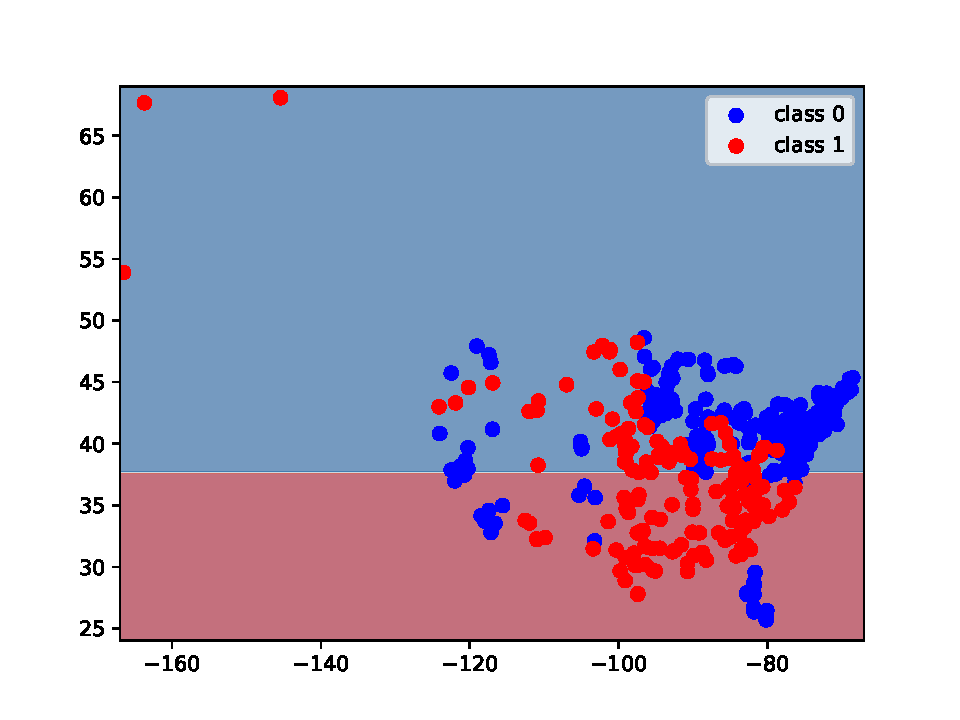
\includegraphics{C:/Users/wangzhen/Desktop/cpsc340/u7p1b_a1/figs/q2_2_decisionBoundary.pdf}
\caption{Decision boundary for inequality}
}

\subsection{Constructing Decision Trees}
\rubric{code:2}

Once your decision stump class is finished, running \texttt{python main.py -q 2.3} will fit
a decision tree of depth~2 to the same dataset (which results in a lower training error).
Look at how the decision tree is stored and how the (recursive) \emph{predict} function works.
\blu{Using the same splits as the fitted depth-2 decision tree, write an alternative version of the predict
function for classifying one training example as a simple program using if/else statements
(as in slide 6 of the Decision Trees lecture).} Save your code in a new file called
\texttt{simple\string_decision.py} (in the \emph{code} directory) and make sure you link to this file from your README.

Note: this code should implement the specific, fixed decision tree
which was learned after calling \texttt{fit} on this particular data set. It does not need to be a learnable model.
\textcolor{gre}{
\\Answer: The URL of the python code is: \url{https://github.ugrad.cs.ubc.ca/CPSC340-2017W-T2/u7p1b_a1/blob/master/code/simple_decision.py}.}

\subsection{Decision Tree Training Error}
\rubric{reasoning:2}

Running \texttt{python main.py -q 2.4} fits decision trees of different depths using two different implementations: first,
our own implementation using your DecisionStump, and second, the decision tree implementation from the popular Python ML library \emph{scikit-learn}.
The decision tree from sklearn uses a more sophisticated splitting criterion called the information gain, instead of just the classification accuracy.
Run the code and look at the figure.
\blu{Describe what you observe. Can you explain the results?}

Note: we set the \verb|random_state| because sklearn's DecisionTreeClassifier is non-deterministic. I'm guessing this is
because it breaks ties randomly.

Note: the code also prints out the amount of time spent. You'll notice that sklearn's implementation is substantially faster. This is because
our implementation is based on the $O(n^2d)$ decision stump learning algorithm and sklearn's implementation presumably uses the faster $O(nd\log n)$
decision stump learning algorithm that we discussed in lecture.
\textcolor{gre}{
\\Answer:
From the figure below,\\ 
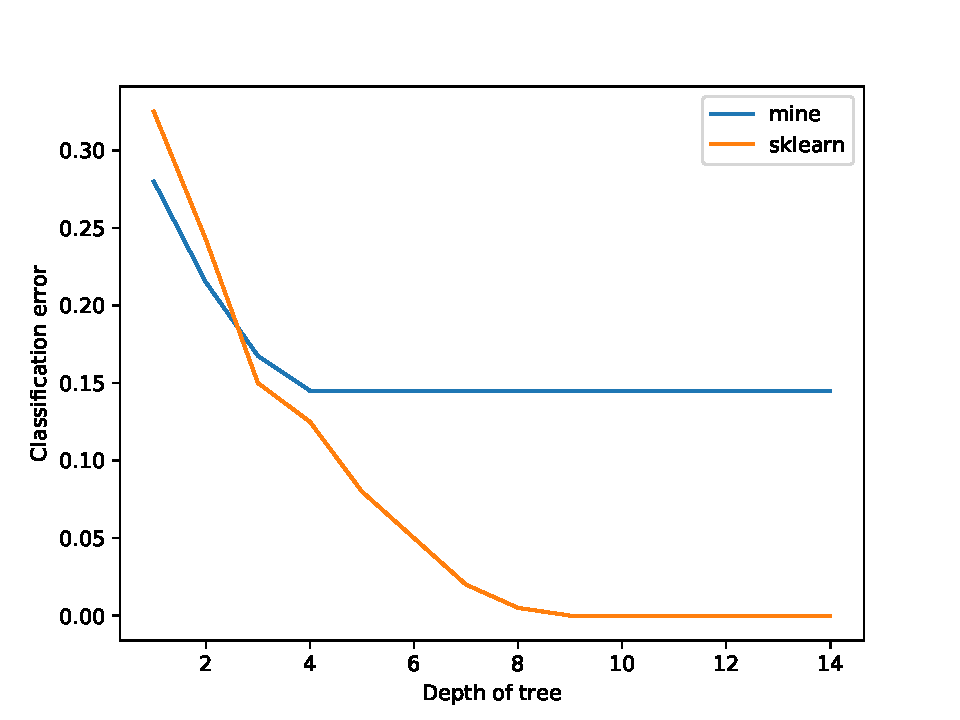
\includegraphics{C:/Users/wangzhen/Desktop/cpsc340/u7p1b_a1/figs/q2_4_tree_errors.pdf}
\caption{Tree errors}
We can find that although when the depth is very small, the error of sklearn's DecisionTreeClassifier might be larger and the two errors show similar trend before error of my DecisionStump gets stable. After the error of my DecisionStump get stable in around 0.15, with depth increasing, the error of sklearn's DecisionTreeClassifier continues to decrease and results in zero after depth reaches 9.
The reason should be that our decision stump does splitting works based on the mode of labels. Thus the split cannot help increase the accuracy when the
modes of labels in two sides are the same.
}


\subsection{Cost of Fitting Decision Trees}
\rubric{reasoning:3}

In class, we discussed how in general the decision stump minimizing the classification error can be found in $O(nd\log n)$ time.
Using the greedy recursive splitting procedure, \blu{what is the total cost of fitting a decision tree of depth $m$ in terms of $n$, $d$, and $m$?}

Hint: even thought there could be $(2^m-1)$ decision stumps, keep in mind not every stump will need to go through every example. Note also that we stop growing the decision tree if a node has no examples, so we may not even need to do anything for many of the $(2^m-1)$ decision stumps.
\textcolor{gre}{
\\Answer:
As the depth is $m$, the total number of decision stumps is $(2^m-1)$. This means that it seams the total cost should be $O(2^mndlog n)$. However, not every stump in this decision tree will need to go through every example. In every stump, there is actually an if/else statement and each example should only choose one stump in each layer. As the depth is $m$, the total cost should be $O(mndlog n)$
}

\section{Training and Testing}
If you run \texttt{python main.py \string-q 3}, it will load \emph{citiesSmall.pkl}.
Note that this file contains not only training data, but also test data, \texttt{X\string_test} and \texttt{y\string_test}.
After training a depth-2 decision tree it will evaluate the performance of the classifier on the test data.\footnote{The code uses the "information gain" splitting criterion; see the Decision Trees bonus slides for more information.}
With a depth-2 decision tree, the training and test error are fairly close, so the model hasn't overfit much.

\subsection{Training and Testing Error Curves}
\rubric{reasoning:2}

\blu{Make a plot that contains the training error and testing error as you vary the depth from 1 through 15. How do each of these errors change with the decision tree depth?}

Note: it's OK to reuse the provided code from part 2.4 as a starting point.
\textcolor{gre}{
\\Answer:
As the plot shown below, the training error decreases to 0 after the depth increases to 9. The testing error also shows decreasing trend. But when the depth increases to 9, it shows a slight increase and stays stable with the value of 0.0835.\\
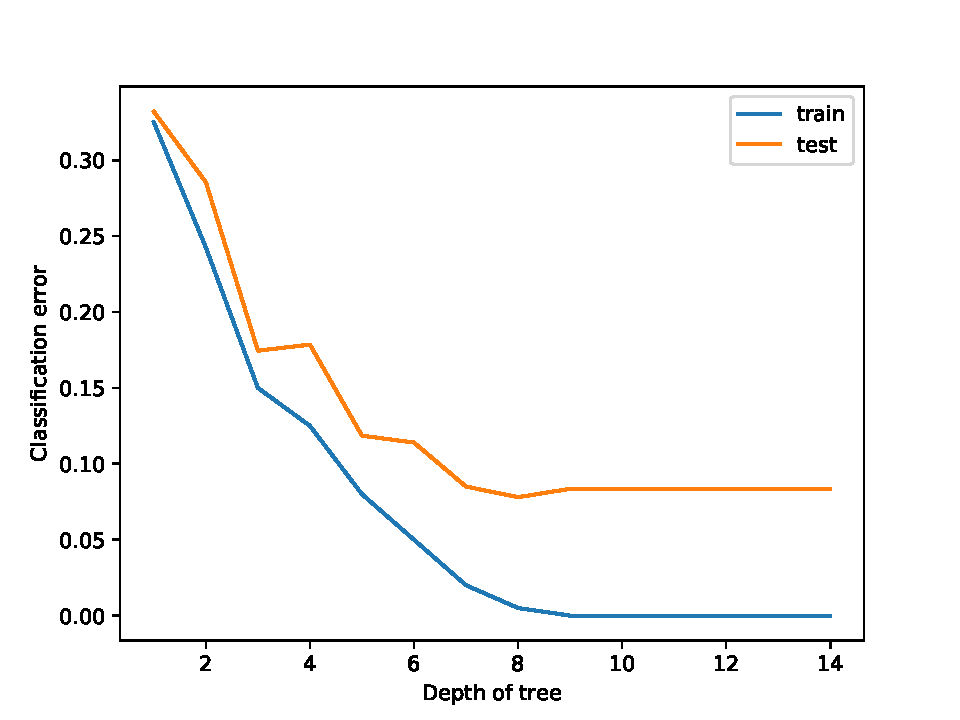
\includegraphics{C:/Users/wangzhen/Desktop/cpsc340/u7p1b_a1/figs/q3_1_train_test_errors.pdf}
\caption{Train and test errors}
}


\subsection{Validation Set}
\rubric{reasoning:3}

Suppose that we didn't have an explicit test set available. In this case, we might instead use a \emph{validation} set. Split the training set into two equal-sized parts: use the first $n/2$ examples as a training set and the second $n/2$ examples as a validation set (we're assuming that the examples are already in a random order). \blu{What depth of decision tree would we pick to minimize the validation set error? Does the answer change if you switch the training and validation set? How could use more of our data to  estimate the depth more reliably?}
\textcolor{gre}{\\
Answer:
The depth is 8 when the validation set error is minimized with the value 0.100. After switch the validation set and the training set, the depth becomes 9 when the minimum validation set error appears as 0.145.
To make it more reliable, we could use cross validation method.\\
The training error and validation error before and after switch is drawn in one graph, the URL is \url{https://github.ugrad.cs.ubc.ca/CPSC340-2017W-T2/u7p1b_a1/blob/master/figs/q3_2_train_vali_errors.pdf}.
}

\section{K-Nearest Neighbours}

In the \emph{citiesSmall} dataset, nearby points tend to receive the same class label because they are part of the same U.S. state. This indicates that a $k$-nearest neighbours classifier might be a better choice than a decision tree. The file \emph{knn.py} has implemented the training function for a $k$-nearest neighbour classifier (which is to just memorize the data).


\subsection{KNN Prediction}
\rubric{code:3, reasoning:4}

Fill in the \emph{predict} function in \emph{knn.py} so that the model file implements the $k$-nearest neighbour prediction rule.
You should Euclidean distance, and may numpy's \emph{sort} and/or \emph{argsort} functions useful.
You can also use \emph{utils.euclidean\_dist\_squared}, which computes the squared Euclidean distances between all pairs of points in two matrices.
\blu{
\enum{
\item Write the \emph{predict} function.
\textcolor{gre}{
\\Answer:The URL of this function is: \url{https://github.ugrad.cs.ubc.ca/CPSC340-2017W-T2/u7p1b_a1/blob/master/code/knn.py}; The URL of the prediction result is: \url{https://github.ugrad.cs.ubc.ca/CPSC340-2017W-T2/u7p1b_a1/blob/master/figs/q4_1_decisionBoundary.pdf}.}
\item Report  the training and test error obtained on the \emph{citiesSmall} dataset for $k=1$, $k=3$, and $k=10$. How do these numbers compare to what you got with the decision tree?
\textcolor{gre}{
\\Answer: when $k=1$, training error=0.0, testing error=0.085; when $k=3$, training error=0.040, testing error=0.055; when $k=10$, training error=0.125, testing error=0.185. Compared with the results from the decision tree, the training error may not be 0 and increase with k increasing. Also, with k increasing, the testing error also shows increase and the value could be larger that that from the decision tree with proper depth.}
\item Hand in the plot generated by \emph{utils.plotClassifier} on the \emph{citiesSmall} dataset for $k=1$, using both your implementation of KNN and the KNeighborsClassifier from scikit-learn.
\textcolor{gre}{
\\Answer: The figure below shows the result of \emph{utils.plotClassifier}:\\ 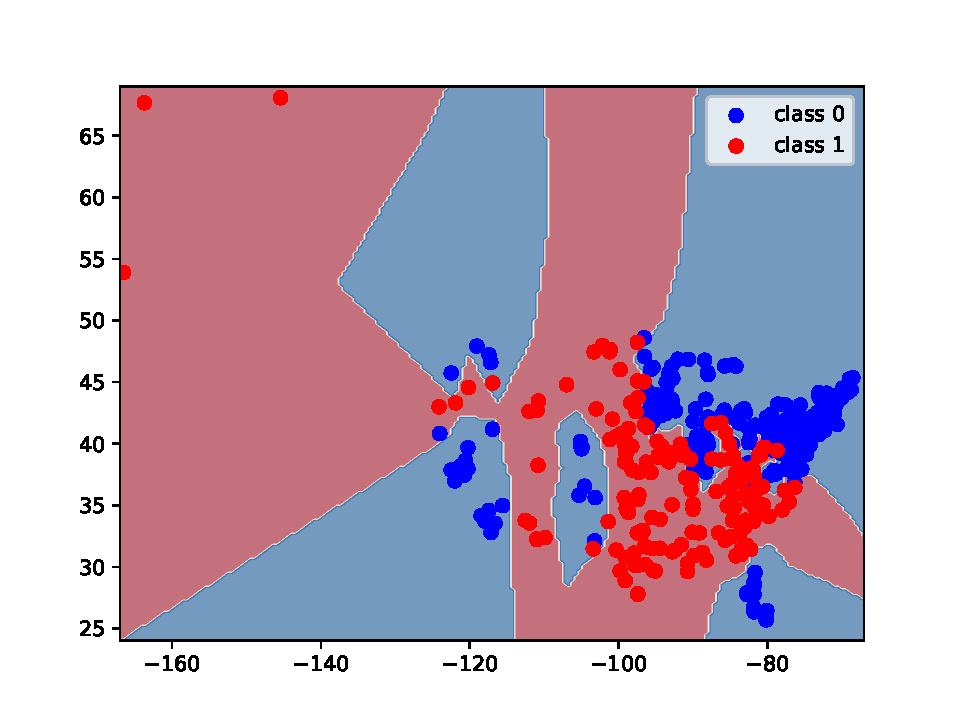
\includegraphics{C:/Users/wangzhen/Desktop/cpsc340/u7p1b_a1/figs/q4_1_decisionBoundarywith.pdf}
\caption{Decision boundary with KNN}
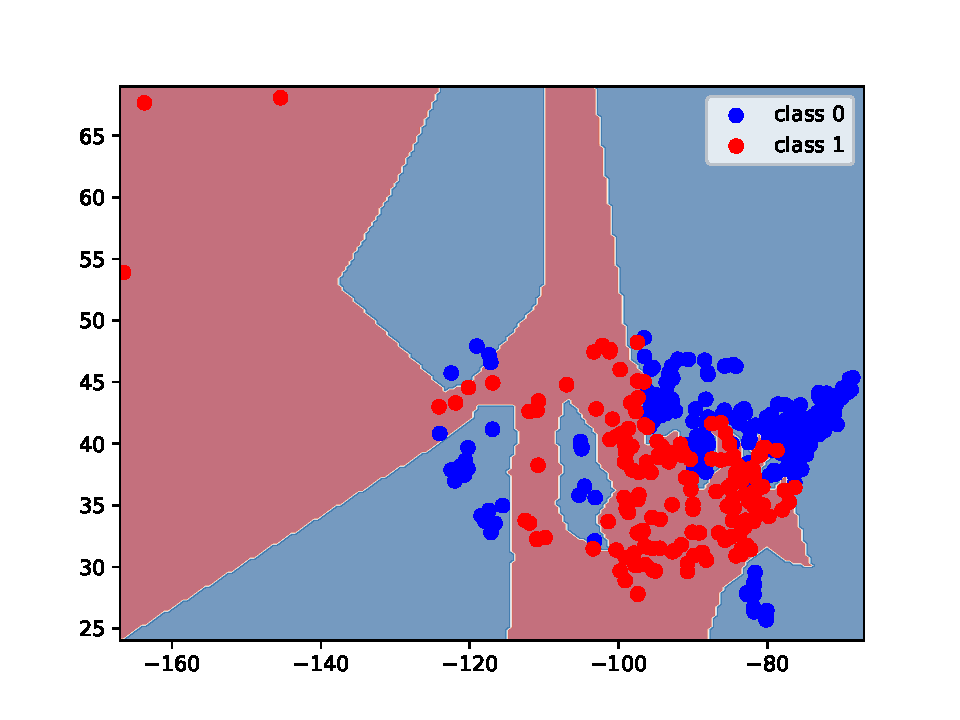
\includegraphics{C:/Users/wangzhen/Desktop/cpsc340/u7p1b_a1/figs/q4_1_decisionBoundarywith_sc.pdf}
\caption{Decision boundary with K-N-Classifier}}
\item Why is the training error $0$ for $k=1$?
\textcolor{gre}{
\\Answer: The training error is 0 when k=1 because every training example is the 1NN of itself. Thus the prediction process is just copy the labels from the training set.}
\item If you didn't have an explicit test set, how would you choose $k$?
\textcolor{gre}{\\Answer: The training error increases as k increases, which means that the training error cannot be used to choose $k$. The method should be to split the data into training and validation set or use cross-validation method.}
}}

\subsection{Condensed Nearest Neighbours}
\rubric{code:3, reasoning:5}

The dataset \emph{citiesBig1} contains a version of this dataset with more than 30 times as many cities. KNN can obtain a lower test error if it's trained on this dataset, but the prediction time will be very slow.
A common strategy for applying KNN to huge datasets is called \emph{condensed nearest neighbours}, and the main idea is to only store a \emph{subset}
of the training examples (and to only compare to these examples when making predictions). If the subset is small, then prediction will be faster.

The most common variation of this algorithm works as follows:

\begin{algorithm}[H]
 initialize subset with first training example\;
 \For{each subsequent training example}{
  \eIf{the example is incorrectly classified by the KNN classifier using the current subset}{
   add the current example to the subset\;
   }{
   do \emph{not} add the current example to the subset (do nothing)\;
  }
 }
 \caption{Condensed Nearest Neighbours}
\end{algorithm}

You are provided with an implementation of this \emph{condensed nearest neighbours} algorithm in \emph{knn.py}.

Your tasks:

\blu{
\enum{
\item The point of this algorithm is to be faster than KNN. Try running the condensed NN on the\\\emph{citiesBig1} dataset and report how long it takes to make a prediction. What about if you try to use KNN for this dataset -- how long did it take before you panicked and went for CTRL-C... or did it actually finish?
\textcolor{gre}{\\Answer: When split the data into 9/10 of training set and 1/10 of validation set, the prediction for training set takes 10.1798s. This is very fast compared to using KNN, which is endless without using Ctrl-C.}
\item Report the training and testing errors for condensed NN, as well as the number of variables in the subset, on the \emph{citiesBig1} dataset with $k=1$.
\textcolor{gre}{\\Answer: The training error is 0.0087; The testing error is 0.0209; The number of variables in the subset is 311.}
\item Hand in the plot generated by \emph{utils.plotClassifier} on the \emph{citiesBig1} dataset for $k=1$.
\textcolor{gre}{\\Answer: The figure below shows the plot:\\ 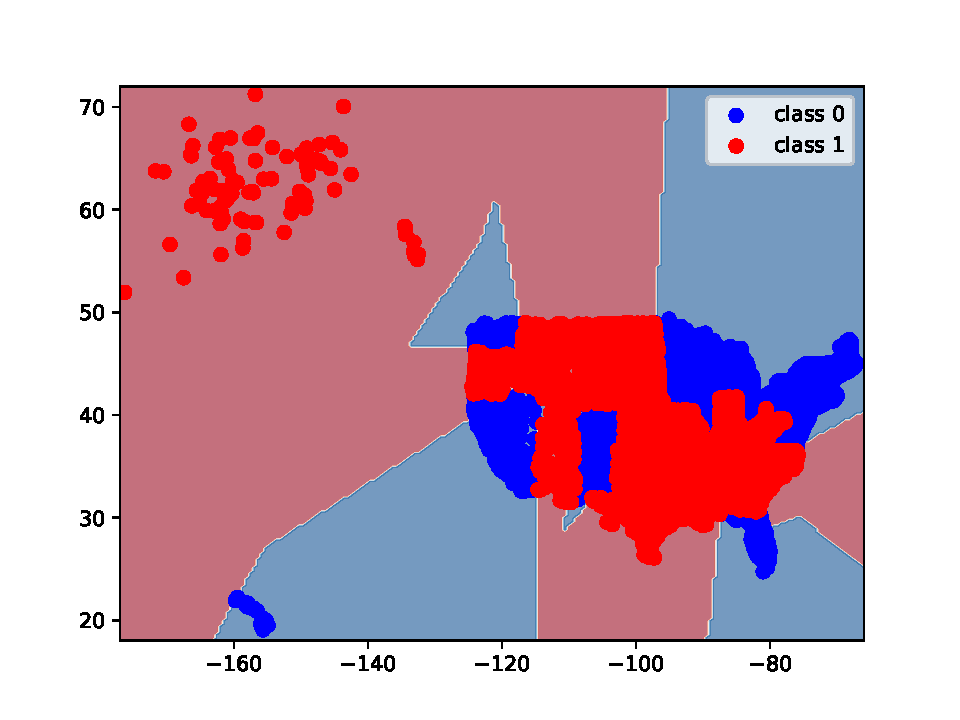
\includegraphics{C:/Users/wangzhen/Desktop/cpsc340/u7p1b_a1/figs/q4_2_decisionBoundary.pdf}
\caption{Decision boundary for CNN}}
\item Why is the training error with $k=1$ now greater than $0$?
\textcolor{gre}{\\Answer: In this case, we do not store examples that were correctly classified during the training phase. When we add more examples to the subset, these examples can become incorrectly classified. We can go through the dataset for more times to fix these errors.}
\item If you have $s$ examples in the subset, what is the cost of running the predict function on $t$ test examples in terms of $n$, $d$, $t$, and $s$?
\textcolor{gre}{\\Answer: Originally we calculate n distances to t test points.But now, we calculate s distances to t test points. Since to calculate one distance takes $O(d)$, the cost is reduced from $O(ndt)$ to $O(sdt)$.}
\item Try out your function on the dataset \emph{citiesBig2}. Why are the  test error \emph{and} training error so high (even for $k=1$) for this method on this dataset?
\textcolor{gre}{\\Answer: In the citiesBig2,the dataset including the training set and the test set is sorted (by state), so the data is not even close to IID. \\The reason that the test error is high: there are some states that are not present in the
training set. \\The reason that the training error is high: the CNN method depends on the
order of the examples thus all the cities in a state might be correctly classified as we visit all at once but
then they can become incorrectly classified since we an try to get
other states right and don't visit them again .}
\item Try running a decision tree on \emph{citiesBig1} using scikit-learn's \texttt{DecisionTreeClassifier} with default hyperparameters. Does it work? Is it fast? Any other thoughts? Overall, do you prefer decicison trees of (condensed) KNN for this data set? Include the usual plot of the decision surface.
\textcolor{gre}{\\Answer: The plot using decision tree is:\\
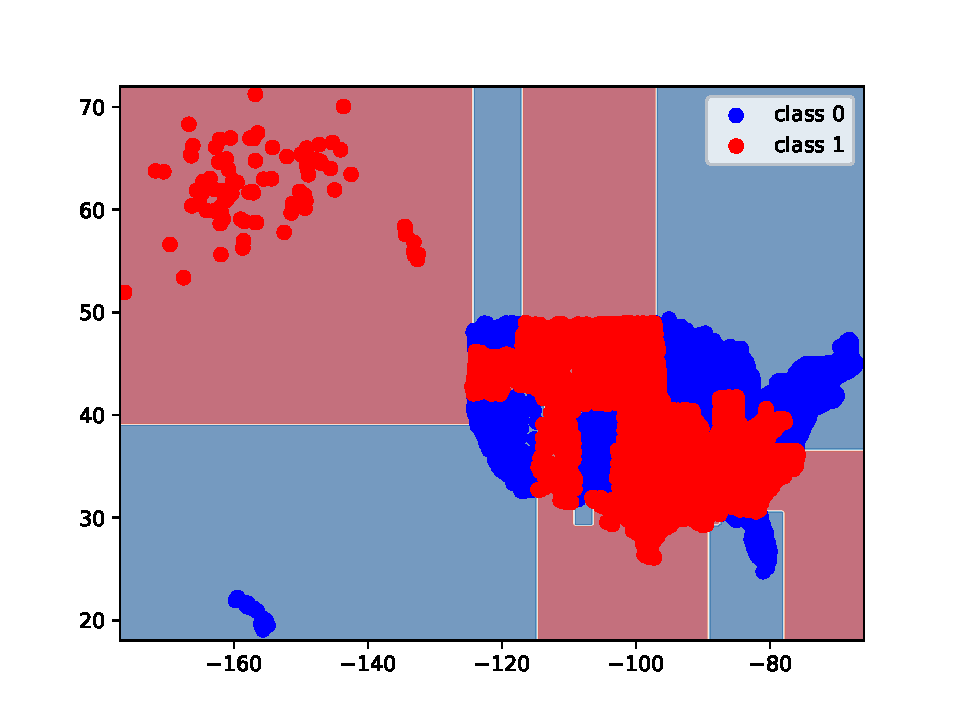
\includegraphics{C:/Users/wangzhen/Desktop/cpsc340/u7p1b_a1/figs/q4_2_Decision_tree_boundary.pdf}
\caption{Decision boundary for decision tree}
The method using the decision tree is pretty faster than using the CNN.And the testing error is smaller (0.013 and 0.025). Thus I prefer the decision tree.}
}
}



\section{Very-Short Answer Questions}
\rubric{reasoning:8}

\blu{Write a short one or two sentence answer to each of the questions below}. Make sure your answer is clear and concise.

\enum{
\item What is one reason we would want to look at scatterplots of the data before doing supervised learning?
\textcolor{gre}{\\Answer: There might be some odd data in the dataset. Or the data might be simple and show obvious features.}
\item What is a reason that the examples in a training and test set might not be IID?
\textcolor{gre}{\\Answer: The examples are sorted. }
\item What is the difference between a validation set and a test set?
\textcolor{gre}{\\Answer: A validation set is a part of the training set and is to use to approximate test error after training. A test set is a set for testing which cannot have any influence on training. A test set may contain new data. }
\item What is the main advantage of non-parametric models?
\textcolor{gre}{\\Answer: The more the data is, the more complicated the model will be. }
\item A standard pre-processing step is ``standardization'' of the features: for each column of $X$ we subtract its mean and divide by its variance. Would this pre-processing change the accuracy of a decision tree classifier? Would it change the accuracy of a KNN classifier?
\textcolor{gre}{\\Answer: For decision tree, it would not as it does not change the relative ordering of the features. For KNN classifier, it would as it changes the importance of each dimension. }
\item Does increasing $k$ in KNN affect the training or prediction asymptotic runtimes?
\textcolor{gre}{\\Answer: No. The runtime is not related to k in this case for both fitting and predicting process. }
\item How does increase the parameter $k$ in $k$-nearest neighbours affect the two parts (training error and approximation error) of the fundamental trade-off (hint: think of the extreme values).
\textcolor{gre}{\\Answer: Increasing k will increase the training error but decrease the approximate error. }
\item For any parametric model, how does increasing number of training examples $n$ affect the two parts of the fundamental trade-off.
\textcolor{gre}{\\Answer: Increasing n will lead to a relatively high training error and decrease the approximate error. }
}


\end{document}
